\documentclass{standalone}
\usepackage[T1]{fontenc}
\usepackage[utf8]{inputenc}          % needed for French accents
\usepackage{pgfplotstable}
\usepackage{pgfplots}
\pgfplotsset{compat=1.18}
\usepackage{siunitx}                 % optional, nicer y‑axis numbers
\usepackage{booktabs}                % pretty tables for the optional preview

% -------------------------------------------------
% Helper that removes the internal \pgfpl@@ wrapper
% -------------------------------------------------

\begin{document}
% This file was created with matplot2tikz v0.4.0.


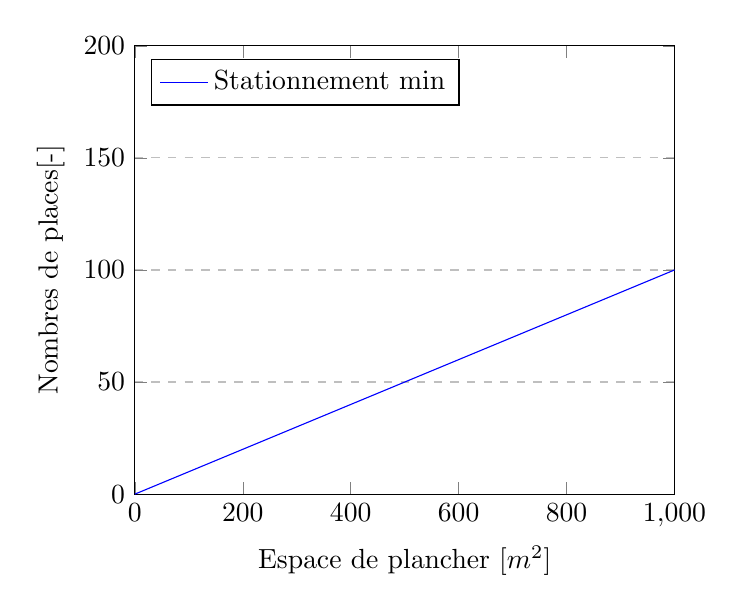
\begin{tikzpicture}
    \begin{axis}[
        xlabel={Espace de plancher [$m^2$]},
        ylabel={Nombres de places[-]},
        xmin=0, xmax=1000,
        ymin=0, ymax=200,
        xtick={0,200,400,600,800,1000},
        ytick={0,50,100,150,200},
            legend pos=north west,
        ymajorgrids=true,
        grid style=dashed,
    ]
        \addplot[
            color=blue
            ]
        coordinates {
        (0,0)(500,50)(800,80)(1000,100)
        };
        \legend{Stationnement min}
    \end{axis}
\end{tikzpicture}


\end{document}